\section{Combination into a Process-Driven Semi-Event-Based Micro-service DWS}
\label{sec:finalArchitecture}
After having introduced the basic technologies, this section aims to combine those into the process-driven semi-event-based microservice architecture for data warehouse systems. The focus will be generic and lies within the interaction between multiple components. There will not be any detailed choice of various processes or products. To verify its usability and feasibility, an evaluation from industrial point of view will be appended. This will be achieved by interviewing a technical expert.

\subsection{Introducing the Process-Driven Semi-Event-Based Microservice Approach for Data Warehouse Systems}
\begin{figure}[!htb]
    \centering
    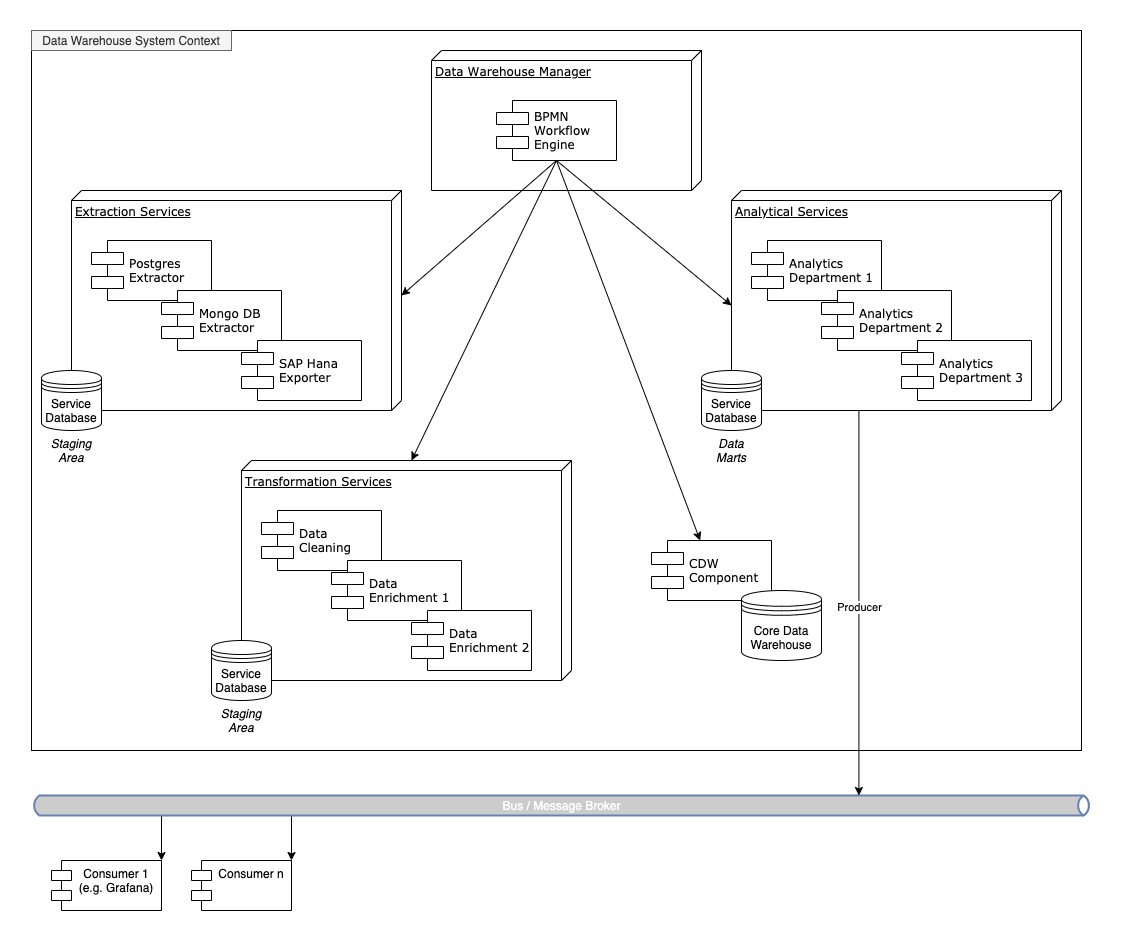
\includegraphics[scale=0.43]{pictures/ResultingArchitecture.png}
    \caption{Process-driven semi-event-based microservice architecture for data warehouse systems}
    \label{fig:resultingArch}
\end{figure}
Figure \ref{fig:resultingArch} shows the resulting architecture. In the next paragraph we will have a more detailed summary of the components and their interactions.\newline
\\
Starting off with the data warehouse manager which contains a BPMN workflow engine used for the orchestration of the whole system. Additionally, all information of the process flow is stored and maintained within this component. \newline
Next, let us focus at the service cluster for data extraction. It contains microservices as SCS which are controlled via the data warehouse manager. As shown in the diagram, each service has its own database. Typically, in the extraction layer the staging area is used as temporary data storage.  It can be thought of having distinct services depending on the input format. Nevertheless, there are multiple other possibilities about how to split up this component. As mentioned within chapter \ref{sec:techKnowHow} it is recommended to slice the services along the process which is defined within the BPMN diagram.\newline
Besides of that, the transformation services are orchestrated by the workflow engine as well. They get cascaded as needed within the BPMN diagrams. As shown in the cluster, data cleaning, cleansing and enhancement is provided. These self-contained systems will hand over the data into a CDW component which stores the historical data.\newline
In the cluster for analytical services, there are multiple instances which are used to extract and store a subset of data within data marts. Due to the orchestration done by BPM, it is possible to cascade multiple services in order to make department specific analysis possible. Furthermore, the information will be shared via a message broker or event bus system with various consumers which are often run by departments. As shown within the picture, it would be possible to use \acrshort{bi} self-services like Grafana or Tableau to generate reports from that information.\newline
\\
In conclusion, the key features are contained within the SCS approach to DWS, the process-driven orchestration using a BPMN workflow engine as well as the data supply via an event bus / message broker. By making use of these principles the overall systems get more adaptive in terms of customer needs. The overall development and dependency management gets easier and faster. 

\subsection{Evaluation of this Architecture from an industrial Point of View}
To verify the feasibility, the purpose and the improvements of this approach in contrast to the presented ones in chapter \ref{sec:referenceArchitecture} and \ref{sec:otherArchitectures} an interview is conducted. Before introducing the outcome guidelines and candidates need to be defined and chosen.

\subsubsection{Guidelines for the Interview}
These guidelines aim to define questions which should be answered by consulted experts. The overall aim is to ensure the benefits of this approach as well as en-lighting some weaknesses. 
\begin{itemize}
    \item Can a benefit be seen within the adaptive orchestration of microservices by applying BPM?
    \item Does the use of self-contained systems make sense in this field of application?
    \item Is this approach overall more beneficial than the introduced ones by Kimball and Inmon?
    \item What are possible weaknesses or bottlenecks within the introduced architecture?
\end{itemize}

\subsubsection{Selection of Proper Candidates}
In order to have meaningful feedback, two candidates will be chosen. Due to the area of research, it is an obvious choice to select two software / system architects with a lot of experience.\newline
\\
In terms of software architecture, Dr. Dirk Nitsche is going to evaluate the resulting systems and the underlying architectural paradigms. He did his PhD in the area of database and knowledge systems at the Technical University of Munich and is currently employed as a software architect at Siemens Mobility. Due to his knowledge in data driven applications and expertise in this area, he was selected for this evaluation.\newline
Dr. Hanno Walischewski is taking over from the systems point of view. He achieved his PhD in 1999 at the University of Freiburg concerning the learning and understanding of structured documents. Afterwards, he made his way into systems architecture and is currently Chief Architect for Intelligent Traffic Systems at Siemens Mobility. He has great know-how in terms of microservices and their collaboration. Due to this, he will analyse the orchestration of those services and their weaknesses.

\subsubsection{Resulting Feedback}
\cite{dirk}\newline
\\
''This approach goes nicely the same way as may other architecture refactorings nowadays: splitting monoliths into a set of microservices. The classical way a data warehouse system was one big block that did all the work like a black box. Decoupling this into smaller pieces follows the learnings over the last years. Scalability can be realized in a much more detailed way depending on the use cases that shall be covered.\newline
The microservice design results in simpler components, but lifts more complexity into the network and communication layer. Using a BPMN engine to orchestrate the involved components helps avoiding the implementation of complex pattern like saga (https://microservices.io/patterns/data/saga.html).\newline
For future work it is definitely worth implementing a proof of concept to show the strength of  this approach. Due to the success of a lot of other migrations from monolithic to distributed architectures, it can be expected to be more flexible and performant.'' \cite{hanno}